%%%%%%%%%%%%%%%%%%%%% chapter2.tex %%%%%%%%%%%%%%%%%%%%%%%%%%%%%%%%%
%
% sample chapter
%
% Use this file as a template for your own input.
%
%\motto{Use the template \emph{chapter.tex} to style the various elements of your chapter content.}
\chapter{Level of Service - Impact Hierarchy}
\label{2:los} % Always give a unique label
% use \chaptermark{}
% to alter or adjust the chapter heading in the running head
\chapterauthor{Bryan T. Adey and Nam Lethanh}
\section{General}
In order to determine what to do with infrastructure it is necessary to determine what is expected from the infrastructure, i.e. it is necessary to determine the required LOSs. This must be defined for a specific time period. It requires the determination of an impact hierarchy and the determination of the values of each impact indicator or impact value over the specified period of time \citep{Adey2012}.
\section{Impact hierarchy - Theory}
\subsection{General}
The best way to define LOS provided by infrastructure is to consider it to be identical to the amount that persons are affected by the functioning (or non-functioning) of infrastructure with respect to the required LOS. For example, on a road network, it may be expected that next year $x$ $mus$\footnote{$mus$ stands for monetary units} are to be spent on the execution of maintenance interventions and y mus worth of impacts are due to accidents. If more than $x$ $mus$ are to be spent on maintenance and more than $y$ $mus$ worth of impacts occur due to accidents than it can be considered that an inadequate LOS was provided. If less or equal, than it can be considered that an adequate LOS was provided.

If it is too difficult to quantify all impacts to be used to measure LOS in terms of directly comparable units (above they are given in $mus$) proxies can be used. For example, instead of stating that y mus worth of impacts due accidents are expected next year, the number of accidents may be stated. 

The type of proxy used can be evaluated with respect to its usefulness in assessing the amount that persons are affected by the functioning (or non-functioning) of infrastructure with respect to the required LOS. For example, the number of accidents might be considered a relatively good proxy with respect to the amount persons are affected by accidents, whereas the number of potholes in the road, might not be. The number of accidents can be multiplied by the average impact of an accident to give the expected total impacts, whereas if the number of potholes is used to calculate the expected total impact, it must be multiplied with the expected number of accidents that occur when there are this number of and the average impact of an accident \footnote{the expected number of accidents when a road section has $x$ numbers of potholes is often estimated as probabilistic function that takes into account of some factors such as numbers of potholes, traffic volume, vehicle speed, etc.}. In general, the fewer the number of calculations that are required to determine the amount that persons are affected, the better.

In any case, the determination of the values of the proxies to be used should be approximated based on a rigorous assessment of the impacts related to these values, and a comparison of these values with the other impact types used to define LOS. If not, an optimal performance of the infrastructure will not be targeted.

It is important to define the LOS so that it covers all ways in which persons can be affected by the functioning (or non-functioning) of infrastructure. If this is not done, then there is a significant probability that managers will concentrate on some impacts and ignore others, which may also be important. For example, a manager might choose to reduce the probability of occurrence of an accident in a tunnel to a very small amount by imposing a regulation to reduce vehicle speed (e.g. from 100 km/hour to 80 km/hour) in the tunnel if only owner costs and accident costs are considered. If, however, owner costs, the costs of travel time and the costs of accidents are taken into consideration he may determine that the best strategy is to renew the road surface and the lighting system more frequently, even though it would result in higher costs for the owner.

To ensure that all this can be done it is useful to:

\begin{itemize}%[leftmargin=2pt-.8in]
\item determine the objective of setting the LOS
\item determine and classify the persons affected by the functioning (or non-functioning) of the infrastructure, i.e. stakeholders
\item determine and classify the ways in which each of the stakeholders are affected, i.e. the impact types. 
\item determine the indicators to be used to determine the value of the impacts incurred by stakeholders,
\item determine the value of a unit change in the indicators used in units that can be compared across all impact types.                                                                                                                    \end{itemize}


The grouping of stakeholders, their impacts at each level, and the indicators to be used to measure these impacts are referred to as an impact hierarchy. In the development of an impact hierarchy it is important that it is: 

\begin{enumerate}
\item \textbf{complete} - all non-negligible ways in which persons are affected should be included. If not, there will be an unwanted focus on the items included in the hierarchy to the detriment of those that are not, which may lead overall to sub-optimal decisions.
\item \textbf{decomposable} - each impact should be broken down, or decomposed, to a level that is reasonable quantifiable. If the hierarchy is not decomposable to a reasonable good quantifiable level persons will be required to place numbers on impacts relatively subjectively.  
\item \textbf{operational} - the impacts should be defined in a way and a level which it is reasonable to quantify them in terms of effort. If a hierarchy is defined in too much detail the effort will be too large to conduct the required analysis or to collect the required information. If a hierarchy is defined in too little detail, there will be so much subjectivity in the assessment of the value of the impacts that the results will be relatively useless. 
\item \textbf{non-redundant, or orthogonal} - the impacts should be defined in a way that ensures impacts are not double counted. To help ensure orthogonality it is sometimes helpful to make use of the pillars of sustainability, i.e. economic, environmental, and social, in the definition of the lowest level impacts in the hierarchy. If the hierarchy is not orthogonal than the double counting of some, but not all, of the impacts will result in overall sub-optimal decisions.                                                                                                                                                                                                                                                                                                                                                                                                                                                                                 \end{enumerate}
%
\subsection{Objective}
The stakeholders, impacts types and proxies to be considered depend on the objective of determining the LOS. For example, if a road manager wants to determine the work program that will maximize the net positive impact that society as a whole obtains from the infrastructure, only changes that are relevant to society as a whole are considered, and therefore positive impacts on one stakeholder that are negative impacts on another are not taken into consideration. For example, the income that is received from charging a toll on a public road would not be considered as it is a positive impact on the owner but a negative impact of equal magnitude on the user.
%
\subsection{Stakeholder}
There are many ways to classify these persons. It is, however, advantageous to group them keeping in mind how models will be built to assess how they are affected over time. For example, a person affected by noise who is driving a car may not be affected in the same way as a person who lives next to road on which cars pass.

Being a stakeholder is time dependent. For example, when a person is driving a vehicle on a road he is a user at that point in time, but when he is off of the road and in his house far from the road he is part of the indirectly affected public. Although he is the same person he is affected by the road when he is using it in one way, and when he is not using it in another way.

Depending on the objective it can be helpful to classify stakeholders as either first level, or second level or third level stakeholders. The first level stakeholders are those whose net positive impacts should be maximized. The second level stakeholders are those whose impacts are the outcome of the maximization of the net impacts of the first level stakeholders, and should be monitored.  The third level of stakeholders are those whose impacts are of no concern.
%
\subsection{Impact}
Each stakeholder can be affected by the functioning (or non-functioning) of the infrastructure in different ways. For example, someone driving on a road can be affected by being in an accident or through the amount of time they spend traveling. 

The impacts are attributed to the stakeholder who is most directly affected. For example, the money spent to hire persons to execute an intervention on a bridge should be attributed to the owner of the bridge rather than the tax payers.

The impact are to be grouped in a hierarchy and given to a level of detail in a way in which it can be reasonably expected that they can be quantified. 

The impact hierarchy should include all non-negligible impacts to the “principal” stakeholders of public road infrastructure, i.e. those whose positive impacts should be maximized. 

\subsection{Indicator}
In order to estimate the impacts it is necessary to determine impact indicators, which are considered to be representative of each impact type. It is only by estimating the values of these indicators over time, and attributing monetary values to each unit change in the indicators, that the impact on the stakeholders can be correctly evaluated. If the values of these indicators are used directly to set a LOS they are referred to as proxies.

\subsection{Conclusions}
Determination of the impact hierarchy is the precursor to setting the required LOS. It is important that sufficient time be spent to define it well, and to ensure that decision makers understand it. It is only with this understanding that the statement of the required LOS will make sense, which will set the stage for good decision making in the future.

Ideally the determination of the required LOS would be closely linked to the theoretically optimal LOS, i.e. the stakeholders as a whole receive the maximum net benefit from the infrastructure. As there are, however, many different stakeholders affected by the functioning (or non-functioning) of infrastructure, with many different opinions of the values to be associated with the unit changes in different types of impacts, the fixing of the required LOS is something that is associated with considerable negotiation between all involved stakeholders \citep{Brauers204}.

\section{Impact hierarchy - an example}
\subsection{Question A}

Develop an impact hierarchy that will allow a public road manager to determine the work program that will maximize the net positive impact that society as a whole obtains from the infrastructure over the next 20 years. Be clear as to the objective of developing the impact hierarchy. Explain the main components of the hierarchy in general. Give the complete hierarchy. Explain how you would attempt to quantify each impact type at the lowest level. 

\subsection{Answer A}

\label{GrindEQpgref4d79f6d52}\subsubsection{Objective}

This impact hierarchy is developed for public roads assuming that a road manager wants to determine the work program that will maximize the net positive impact that society as a whole obtains from the infrastructure Therefore, only changes that are relevant to society as a whole are considered, i.e. positive impacts on one stakeholder that are negative impacts on another are not taken into consideration. For example, the income that is received from charging a toll on public road is not considered as it is a positive impact on the owner but a negative impact of equal magnitude on the user.

\subsubsection{Components}

The impact hierarchy is to consist of stakeholders, impact types and impact indicators.


\paragraph{\underline{Stakeholders}}

A stakeholder is considered as an individual, group, or organization, which is affected by changes to public roads. Being a stakeholder is time dependent, i.e. when a person is driving a vehicle on a road he is a user at that point in time. When he is off of the road and in his house far from the road he is part of the indirectly affected public. It is considered that all stakeholders can be grouped as either first level or second level stakeholders. The first level stakeholders are those whose net positive impacts should be maximized. The second level stakeholders are those whose impacts are the outcome of the maximization of the net impacts of the first level stakeholders, and should be monitored. 

The four first level stakeholder groups are the owner, the user, the directly affected public (DAP), and the indirectly affected public (IAP). It is assumed that all impacts to be maximized can be attributed to one of these four stakeholder groups. The impacts are attributed to the stakeholder who is most directly affected. The definitions of each stakeholder group are given in later parts of this section. 

The proposed impact hierarchy is to be used to take into consideration all non-negligible impacts to the ``principal'' stakeholders of public road infrastructure, i.e. those whose positive impacts should be maximized. It is considered that all people at a point in time can be divided into one of four stakeholder groups, the owner, the user, the directly affected public, and the indirectly affected public. The impact types in the hierarchy are given to a level of detail in which they could be reasonably expected to be quantified. To help ensure orthogonality the pillar of sustainability, i.e. economic, environmental, social, is stated for each of the lowest level impacts. An example of each impact type is given.

\begin{table}[htbp]
\caption{Stakeholders}
\begin{tabular}{|p{90pt}|p{170pt}|p{170pt}|}
\hline
Stakeholders & Definition & Examples \\ \hline
Owner & the persons who are responsible for decisions with respect to physically modifying the infrastructure & a federal road authority  \\ \hline
Users & the persons who are using the roads & a driver and passengers of a vehicle on a road. \\ \hline
Directly affected public & the persons who are in the vicinity of the road but are not using it & persons in a house next to the road that hear vehicles driving on the road. \\ \hline
Indirectly affected public & the persons who are not in the vicinity of the road but are affected by its use & persons in a house far away from the road that do not hear vehicles driving on the road, but are affected by a changing climate due to the emissions produced by vehicles driving on the road. \\ \hline
\end{tabular}
\label{tbl:21}
\end{table}

Second level stakeholder groups, such as contractors, financial institutions, and operators are not considered further than they are considered when considered as one of the above listed stakeholders. The impacts on these stakeholder groups are only the outcome of our efforts to maximize the positive net impact of the four first level stakeholders in the first level.

\paragraph{\underline{Impact types}}

The impacts on each stakeholder are grouped as impact types. The impact types are subdivided at increasingly fine levels until the impact of each type can be reasonably and objectively quantified and modelled. To help to ensure orthogonality in the impact hierarchy, each impact type, on the lowest defined level, is explained and classified as contributing to one of the pillars of sustainability (economic, societal, environmental). An example is given for each to help clarify its meaning. 

\paragraph{\underline{Impact indicators}}

Impact indicators, which are considered to be representative of each impact type are given for each impact type. By estimating the values of these indicators over time, and attributing monetary values to each unit change in the indicators, it is possible to evaluate the impact of the stakeholders. Examples of models to be used to estimate how their values change over time per impact type are given in section 5. The impact hierarchy is given in Table \ref{tbl:22} to Table 5 in the following sections.

\subsubsection{Impact hierarchy}

\paragraph{\underline{Owner}}

The impacts attributed to the owner are grouped as intervention costs (Table \ref{tbl:22}), i.e. the impact on the owner of executing interventions. The impact indicators are the amount of labour, the amount of equipment, and the amount of material to be used to execute interventions, $I_{labor}^o$\textit{,,}$I_{material}^o$ e.g. intervention \textit{w} required \textit{x} man-hours, \textit{y} generator-hours and \textit{z} kilograms of material\footnote{Throughout the document, I represents ``impact'' and it is used to as mathematical notation in functions where appropriate.}. 

The monetary value placed on the 

\begin{itemize}
	\item labor used represents the economic impact of persons performing tasks, i.e. the value from society's perspective of the person doing the intervention. 
	\item material used represents the economic impact of people ensuring that materials are available for use, i.e. the value from society's perspective of persons preparing the materials for use. 
	\item equipment used represents the economic impact of people ensuring that equipment is available for use, i.e. the value from society's perspective of persons preparing the equipment for use.
\end{itemize}

The estimation of the value of an intervention is often done using one of two approaches:

\begin{itemize}
	\item a disaggregate approach where expenditures for each item or activity are estimated and summed. When this approach is used the work break down structure of the intervention project it is often used.
	\item an aggregate approach where sum of all expenditures is estimated directly. An aggregate approach often includes regression analysis and historical information. 
\end{itemize}

\begin{table}[htbp]
\caption{Owner impact types}
\begin{tabular}{|l|p{100pt}|p{70pt}|p{170pt}|}
\hline
\multicolumn{2}{|l|}{Level 1} & \multicolumn{2}{l|}{Level 2} \\ 
\hline
Label & Description & Label & Description \\ 
\hline
Intervention & the impact of executing interventions & Labor* & the economic impact of people performing tasks \\ 
\cline{3-4}
 &  & Material* & the economic impact of people ensuring that materials are available for use \\ 
\cline{3-4}
 &  & Equipment* & the economic impact of people ensuring that equipment is available for use \\ 
\hline
\end{tabular}\\
\label{tbl:22}
\footnotesize * These could be further subdivided based on the type of activity performed, e.g. administration, planning, etc...
\end{table}


\paragraph{\underline{User}}

During the interventions, users experience inconveniences such as traffic jams, bumping condition of temporarily roads (detour roads). The unfavorable conditions of traveling via the road sections and links subjected to intervention will eventually lead to higher possibility of accidents, various types of physical exhaustion and illness as comfort levels decrease, loss of travel time, and increases in fuel consumption and frequency of the maintenance of vehicles.

In between interventions, deterioration processes result in a worsening condition of any infrastructure object. The increasingly poor condition of infrastructure also results in a change in how stakeholders are affected e.g. increases in the number of accidents, travel time, the costs of operating and maintaining vehicles.

The impacts attributed to the user are grouped as: safety, operation efficiency, operation quality, and environment preservation (Table \ref{tbl:23}). 

\begin{table}[htbp]
\caption{User impact types}
\begin{tabular}{|p{70pt}|p{100pt}|p{70pt}|p{150pt}|}
\hline
\multicolumn{2}{|l|}{Level 1} & \multicolumn{2}{l|}{Level 2} \\ 
\hline
Label & Description & Label & Description \\ 
\hline
Safety & the impact on the user due to the user being involved in an accident & property damage & the economic impact of repairing the vehicle \\ 
\cline{3-4}
 &  & injury & the societal impact due to the injury \\ 
\cline{3-4}
 &  & death & the societal impact due to death \\ 
\hline
Operation efficiency & the impact of travel in terms of time required & work & the economic impact of wasting work time traveling \\ 
\cline{3-4}
 &  & leisure & the economic impact of wasting leisure time traveling \\ 
\cline{2-4}
 & the impact of travel in terms of vehicle costs & operation & the economic impact of people ensuring that fuel and oil is available for use \\ 
\cline{3-4}
 &  & maintenance & the economic impact of people repairing vehicles and ensuring that materials, e.g. tires and brake pads, are available for use \\ 
\hline
Operation quality & the impact of traveling on the user & physical & the societal impact of obtaining for example, bruises from an extremely bumpy ride \\ 
\cline{3-4}
 &  & psychological & the societal impact of having for example, anxiety due to a perceived increase in the probability of being involved in an accident, or of seeing things while traveling. \\ 
\hline
Environment preservation (reduction of noise) & the societal impact due to the user coming in contract with sound emissions &  &  \\ 
\hline
\end{tabular}\label{tbl:23}
\end{table}



\begin{enumerate}
 \item Safety (Accidents)
 
 Accidents result in damage to the property of involved parties. The owners will often repair the damaged objects so as to provide adequate service to users after accidents (this would be attributed to the owner). The users, however, will be required to repair their vehicles, and will also be affected by any injury and of course, death, that may befall them. The safety impact type attributed to the user is subdivided into property damage, injury and death impact types.
 \item Property damage
 
  The property damage impact type represents the economic impact of repairing the vehicle, i.e. of providing the user with a functioning mode of transport similar to the one being used before the accident, e.g. the costs of the labor, materials and equipment required to replace the bumper on a vehicle that has been in an accident. The impact indicators for property damage are the amount of labor and materials used to repair vehicles damaged in an accident, expressed as the property damage costs given by $I_{acc - pd}^u$. The value of this impact type can be approximated using the receipts from past repairs.
\item Injury and death

The injury impact type and the death impact type attributed to the user represent the social impact due to injuries and deaths, respectively. They represent the change in interactions between persons that will occur because the user is injured or dead. It is not to be confused with the injury impact type and the death impact type attributed to the directly affected public (refer to section \ref{2dap}) or to the indirectly affected public (refer to section \ref{2iap}). The impact indicators are the number of injuries and deaths incurred in a specified time interval, given by$I_{acc - injury}^u$, $I_{acc - death}^u$, respectively

The value of these impact types can be estimated by using the user's willingness to pay to avoid injury or death. Care must; however, be taken to avoid double counting with the injury impact type and the death impact type attributed to the indirectly affected public. 

\item Operation efficiency

The operation efficiency impact type represents the impact on the traveling of users and on the maintenance and operation of the vehicles. 

\item Travel time

The amount of time traveling on the road is determined by various factors such as: speed, road condition (drivers feel comfortable on a smooth road, and therefore drives faster than on a bumpy road), and the DTV (the daily traffic volume, especially in relation to the road capacity), and road geometry. Furthermore, in case of an intervention, a detour might be needed.

The economic impact of wasting work and leisure time traveling may be thought of as the loss of productivity of the users due to time spent traveling. The impact indicators are the amounts of work and leisure time wasted while traveling and are given by $I_{tt - work}^u$, $I_{tt - leisure}^u$

The value of travel time can be determined using willingness to pay surveys. 

\item Vehicle operation and maintenance

The vehicle operation and maintenance impact types represent the economic impact of people ensuring that fuel and oil is available for use, and the economic impact of people repairing vehicles and ensuring that materials, e.g. tires and brake pads, are available for use, respectively. The impact indicators are$I_{v - oper}^u$$I_{v - main}^u$.

The value of the vehicle operation and maintenance impact types can be approximated using the receipts from fuel and vehicle service receipts.

\item Operation quality

The operation quality impact type is subdivided into the physical and psychological impact types. The physical impact type represents the social impact of obtaining for example, bruises from an extremely bumpy ride. It represents the change in interactions between people that will occur because the physical change in the user due to the bumpy ride. The psychological impact type represents the impact of having for example, anxiety due to a perceived increase in the probability of being involved in an accident, or of seeing things while traveling, e.g. aesthetics. It is believed that any economic impacts relevant to society due to the physical and psychological impacts of traveling, such as the loss of productivity, are negligible, in developed countries. 

The impact indicators are the amounts of physical and psychological impacts of traveling, given by $I_{physical}^u$, $I_{psychological}^u$. 

The value of degrees of bumpiness could be determined through willingness to pay investigations.

\item Environment preservation (noise)

The environment preservation impact type represents the social impact due to the user coming in contact with sound emissions. It is meant to capture the changes that occur in the interactions between people due to sound emissions, e.g. the inability to communicate between driver and passenger while driving.  

The impact indicator is the amount of sound emissions to which the directly affected public is exposed $I_{noise}^u$.

The value of an amount of sound emissions can be determined through willingness to pay investigations.
  
\end{enumerate}

\paragraph{\underline{Directly affected public (DAP)}} \label{2dap}

The impacts attributed to the directly affected public are grouped as: safety, operation quality, and environment preservation (Table \ref{tbl:24}), similar to the impact types of the user. The reason they are handled separately is that the directly affected public is affected in fundamentally different ways than the user. 

\begin{table}
\caption{Directly affected impact types}
\begin{tabular}{|p{70pt}|p{100pt}|p{70pt}|p{150pt}|}
\hline
\multicolumn{2}{|l|}{Level 1} & \multicolumn{2}{l|}{Level 2} \\ 
\hline
Label & Description & Label & Description \\ 
\hline
"Safety & the impact on the directly affected public due being involved in an accident & property damage & the \underline{economic} impact of repairing the vehicle \\ 
\cline{3-4}
(Accidents) &  & injury & the \underline{societal} impact due to the injury \\ 
\cline{3-4}
 &  & death & the \underline{societal} impact due to death \\ 
\hline
Operation quality & the impact of traveling on the directly affected public & physical & the \underline{societal} impact of experiencing vibrations in a building next to a road \\ 
\cline{3-4}
 &  & psychological & the \underline{societal} impact of having for example, anxiety due to a perceived increase in the probability of being involved in an accident, or of seeing things while being next to a road. \\ 
\hline
Environment preservation (reduction of noise) & the \underline{societal} impact due to the directly affected public coming in contract with sound emissions &  &  \\ 
\hline
\end{tabular}
\label{tbl:24}
\end{table}


\begin{enumerate}
 \item Safety (Accidents)

The safety impact type is subdivided into property damage, injury and death impact types. 

\item Property damage

The property damage impact type represents the economic impact of repairing damaged property, to the condition it was prior to the occurrence of the accident, e.g. the costs of the labor, and materials required to repair a retaining wall that has been damaged in an accident. The impact indicator is the property damage cost, $I_{acc - pd}^{dap}$.  

The value of this impact type can be approximated using the receipts from past repairs.


\item Injury and death

The injury impact type and the death impact type attributed to the directly affected public represent the societal impact due to injuries and deaths, respectively. They represent the change in interactions between persons that will occur because someone other than the user is injured or dead. It is not to be confused with the injury impact type and the death impact type attributed to the indirectly affected public. The impact indicators are the number of injuries and deaths incurred in a specified time interval, given by$I_{acc - injury}^{dap}$, $I_{acc - death}^{dap}$, respectively

The value of these impact types can be estimated by using willingness to pay of the directly affected public to avoid injury or death. Care must; however, be taken to avoid double counting with the injury impact type and the death impact type attributed to the indirectly affected public. 

\item Operation quality (Comfort)

The operation quality impact type is subdivided into the physical and psychological impact types. The physical impact type represents the societal impact of obtaining for example, discomfort through vibrations that occur due to road use. It represents the change in interactions between persons that will occur because the physical change in the directly affected public. 

The psychological impact type represents the social impact of having for example, anxiety due to a perceived increase in the probability of being involved in an accident, or of seeing the infrastructure, e.g. aesthetics. It is believed that any economic impacts to be attributed to the directly affected public due to the physical and psychological impacts of others traveling, such as the loss of productivity, are negligible. 

The impact indicators are the amounts of physical and psychological impacts of traveling, given by $I_{physical}^{dap}$, $I_{psychological}^{dap}$. 

The value of degrees of bumpiness can be determined through willingness to pay investigations.

\item Environment preservation (Noise)

The environment preservation impact type represents the social impact due to the directly affected public coming in contact with sound emissions. It is meant to capture the changes that occur in the interactions between people due to sound emissions, e.g. the necessity to change where people meet due to excess noise.  

The impact indicator is the amount of sound emissions to which the directly affected public is exposed $I_{noise}^{dap}$.

The value of an amount of sound emissions can be determined through willingness to pay investigations.
\end{enumerate}
%
\paragraph{\underline{Indirectly affected public (IAP)}} \label{2iap}
%
The indirectly affected public are those that are affected by roads through other mediums, e.g. a person who is affected by an increase in the temperature of the earth due to the CO$_{2 }$emitted during the execution of an intervention on a road. The impacts attributed to the indirectly affected public are grouped as: safety, socio-economic activity, environment preservation, and environment consumption.  

Table \ref{tbl:25} and Table \ref{tbl:26} list the most common impact types and indicators. It is noted that several impact types, such as gas and particle emission also directly affect the users and directly affected public group. However, it is assumed that these impacts are minimal.

\begin{table}
\caption{Indirectly affected public impact types (safety, socio-economic activity)}
\begin{tabular}{|p{70pt}|p{70pt}|p{70pt}|p{70pt}|p{70pt}|p{70pt}|}
\hline
\multicolumn{1}{|l}{Level 1} &  & \multicolumn{1}{l}{Level 2} &  & \multicolumn{1}{l}{Level 3} &  \\ 
\hline
Label & Description & Label & Description & Label & Description \\ 
\hline
Safety (Accidents) & The impact on the indirectly affected public of accidents occurring on roads & injuries & the economic impact due to an injury &  &  \\ 
\cline{3-6}
 &  & deaths & the economic impact due to a death &  &  \\ 
\hline
Socio-economic activity & The impact on the ...due to changes in socio-economic development & Persons & the impact of not  being able to transport people & Productivity & the economic impact due to not being able to transport people, e.g. a crop cannot be harvested as workers cannot be transported to the field \\ 
\cline{5-6}
 &  &  &  & Health & the societal impact due to injuries and deaths of not being able to get proper medical care \\ 
\cline{3-6}
 &  & Goods & the impact of not being able to move goods & Productivity & the economic impact due to not being able to deliver goods, e.g. because of not being able to work as planned \\ 
\cline{5-6}
 &  &  &  & Health & the societal impact due to not being able to deliver goods, e.g. due to deaths because of lack of food or medical supplies \\ 
\cline{3-6}
 &  & Employment & social and economic impact of interventions in terms of employing people &  &  \\ 
\hline
\end{tabular}
\label{tbl:25}
\end{table}

\begin{table}
\caption{Indirectly affected public impact types (environment preservation, environment consumption)}
\begin{tabular}{|p{70pt}|p{70pt}|p{70pt}|p{70pt}|p{70pt}|p{70pt}|}
%\begin{tabular}{|l|l|l|l|ll|}
\hline
\multicolumn{1}{|l}{Level 1} &  & \multicolumn{1}{l}{Level 2} &  & Level 3 &  \\ 
\hline
Label & Description & Label & Description & \multicolumn{1}{l|}{Label} & Description \\ 
\hline
"Environment preservation & The impact on ... due to the environment being impacted by particle emissions & CO2 & the impact due to the emissions  & \multicolumn{1}{l|}{Production} & the environmental impact of emissions emitted during the production of materials \\ 
\cline{5-6}
(Reduction of gas and particles emissions) &  &  &  & \multicolumn{1}{l|}{Material transport} & the environmental impact of emissions emitted during the transport of materials to and from the construction site  \\ 
\cline{5-6}
 &  &  &  & \multicolumn{1}{l|}{Person transport} & the environmental impact of emissions emitted during travel \\ 
\cline{5-6}
 &  &  &  & \multicolumn{1}{l|}{Health} & the societal impact due to emissions (human health) \\ 
\cline{3-6}
 &  & PM10 & Same as for CO2 &  &  \\ 
\cline{3-3}\cline{5-6}
 &  & nitrogen &  &  &  \\ 
\cline{3-3}\cline{5-6}
 &  & carbon monoxide &  &  &  \\ 
\cline{3-3}\cline{5-6}
 &  & aldehydes &  &  &  \\ 
\cline{3-3}\cline{5-6}
 &  & nitrogen dioxide &  &  &  \\ 
\cline{3-3}\cline{5-6}
 &  & sulphur dioxide &  &  &  \\ 
\cline{3-3}\cline{5-6}
 &  & polycyclic aromatic hydrocarbons &  &  &  \\ 
\cline{3-3}\cline{5-6}
 &  & dust &  &  &  \\ 
\hline
Environment consumption & The impact on ... due to the slower depletion of finite amounts of non renewable  resources & Energy & the environmental impact due to the consumption of energy not related to emissions, e.g. depletion of finite amounts of non-renewable energy sources &  &  \\ 
\cline{3-6}
 &  & Materials & the environmental impact of consuming materials, not related to emissions  &  &  \\ 
\cline{3-6}
 &  & Land & The land impact type represents the environmental impact due to the consumption of land not related to emissions &  &  \\ 
\cline{3-6}
 &  & Culture & The culture impact type represents the societal impact of changing things important to our identity (of which heritage is part) &  &  \\ 
\hline
\end{tabular}
\label{tbl:26}
\end{table}

\begin{enumerate}
 \item Safety (Accidents)
The injury impact type and the death impact type attributed to the indirectly affect public represents the economic impact due to injuries and deaths, respectively. They represent the loss in productivity due to injuries and deaths, respectively. It includes changes to human activity, such as a doctor's time in an emergency room and the time required ensuring that an insurance company conducts the required financial transactions. The impact indicator is the amount of work time lost, when compared to the reference case where the accident had not occurred given by $I_{safety\_time}^{iap}$.

The value of each amount can be determined by estimating the loss of productivity of the person involved in the accident.

\item Socio-economic activity

The socio-economic activity impact type represents the contribution of the road to socio-economic development. It is composed of persons, goods and employment impact types.

\item Persons

The person impact type is further divided into a productiveness impact type and a health impact type. 

\begin{itemize}
\item Productivity

The productiveness impact type represents the economic impact due to not being able to travel, e.g. a farmer cannot harvest his entire crop because he needs to spend a significantly larger portion of his time getting his goods to market. The impact indicator is the amount of lost work, given by $I_{trans - p - wt}^{iap}$, and expressed in units of time. 

The value of each amount can be determined by conducting through simulations of the performance of the region. 

\item Health

The health impact type represents the societal impact due to injuries and deaths that occur due to not being able to obtain standard medical care, due to a shortage of available persons. The impact indicators are the number of injuries and deaths incurred in a specified time interval, given by$I_{trans - p - injury}^{iap}$, $I_{trans - p - death}^{iap}$, respectively. The value of each amount can be determined by conducting through simulations of the region.
\end{itemize}

\item Goods

The goods impact type is also further divided into a productiveness impact type and a health impact type. 

\begin{itemize}
\item Productivity

The productiveness impact type represents the economic impact due to not being able to deliver goods, e.g. a farmer cannot plant his crop on time since fertilizer could not be delivered as planned. The impact indicator is the amount of lost work, given by $I_{trans - g - wt}^{iap}$.and expressed in units of time.

\item Health

The health impact type represents the societal impact due to injuries and deaths due to goods such as food or medical supplies not being delivered as planned, e.g. the change in society that occurs due to the death of someone in a hospital that would not have died if medical supplies had been delivered as planned. The impact indicators are the number of injuries and deaths incurred in a specified time interval, given by$I_{trans - g - injury}^{iap}$, $I_{trans - g - death}^{iap}$, respectively.
\end{itemize}

\item Employment

The employment impact type represents the societal impact of executing interventions in terms of employing people that is not captured by the impact type attributed to the owner due to the execution of interventions or the user due to the maintenance of vehicles used for traveling. It includes economic development. The impact indicator is the amount of work provided given by $I_{work}^{idap}$. 

The value can be estimated as using economic impact assessment models such as those proposed in \cite{cubrc2001}; \cite{Davis2001}; \cite{Kumares2007}, using predictions of business output, value added, employment level, wages and salaries, and wealth are made.

\item Environment preservation (emissions)

The environment preservation (emissions) impact type of the indirectly affected public represents the environmental and societal impact due emissions emitted during the production and transport of materials and persons. 

It is subdivided by particle emitted, e.g. CO$_{2}$, PM10, NO, CO, aldehydes, NO$_{2}$, SO$_{2}$, polycyclic aromatic hydrocarbons and dust. The impact indicators are the amounts of each that are emitted, given by $I_{C{O_2}}^{iap}$., $I_{P{M_{10}}}^{iap}$, $I_{CO}^{iap}$, $I_{aldehydes}^{iap}$, $I_{N{O_2}}^{iap}$, $I_{S{O_2}}^{iap}$, $I_{pah}^{iap}$,  $I_{dust}^{iap}$ .

Each of these are further subdivided into 

\begin{itemize}
	\item[-] the production impact type, which represents the \underline{environmental} impact of emissions emitted during the production of materials
	\item[-] the material transport impact type, which represents the \underline{environmental} impact of emissions emitted during the transport of materials to and from the construction site
	\item[-] the person transport impact type, which represents the \underline{environmental} impact of emissions emitted during travel
	\item[-] the health transport impact type, which \underline{societal} impact due to emissions (human health). It is meant to capture the changes that occur in the interactions between people due the changes in the people, e.g. due to sickness.  
\end{itemize}

The value of each amount can be determined by analyzing historical records or by conducting empirical studies using emission measurement tools and instruments.

\item Environment consumption

The environment consumption impact type represents the depletion of finite amounts of non-renewable resources. It is subdivided into the energy impact type, the material impact type, the land impact type and the culture impact type.

\begin{itemize}
\item Energy

The energy impact type represents the environmental impact due to the consumption of energy not related to emissions, e.g. depletion of finite amounts of non-renewable energy sources. The impact indicator is a measure of the significance of a unit depletion of a finite resource, given by $I_{energy}^{iap}$.

\item Material

The material impact type represents the environmental impact of consuming materials, not related to emissions, e.g. the consumption of wood has an impact on woodland areas. The impact indicator is the amount of consumed material, e.g. kg of wood cut, given by $I_{materials}^{iap}$. 

\item Land

The land impact type represents the environmental impact due to the consumption of land not related to emissions, e.g. increased environmental damages due to floods. The impact indicator is the m$^{2}$ of land converted from a natural state to a built state, given by $I_{land}^{iap}$. 

\item Culture

The culture impact type represents the societal impact of changing things important to our identity (of which heritage is part).The impact indicator is a measure of the significance of an object to our identity, given by $I_{culture}^{iap}$. The value can be estimated through willingness to pay investigations. 
\end{itemize}

\end{enumerate}

\subsection{Question B}

In reading such an impact hierarchy some people will imagine things that may seemingly not be in the list of impacts. To help clarify this, explain why your impact hierarchy does not include an impact type ``access'' or an impact type ``natural hazard risk''.

\subsection{Answer B}

\subsubsection{Access}

The improvement of access is often stated as an impact \citep{Kumares2007}. Improved access, however, is a proxy for the many things that actually happen when access is improved. For example, if access to a highway is improved a user traveling from point A, to point B, who normally would not take the highway, would perhaps have a shorter travel time, reduced vehicle costs, and reduced accident costs. It is proposed that if it is desired to approximate the value of improved access that the changes in the relevant impact types for each stakeholder are calculated. 

A more numeric example is as follows (Table \ref{tbl:27}). If there are two interventions being considered for a highway (intervention A with a medium level of access and intervention B with a high level of access), it is possible that intervention B will result in a shorter distance for users to travel to arrive at their destinations in comparison with intervention A. This in turn results in a reduction in:

\begin{itemize}
	\item[-] accident costs of 2 mus, 
	\item[-] comfort costs of 5 \textit{mus},
	\item[-] travel time costs of 4 \textit{mus}, and
	\item[-] vehicle costs of 2 \textit{mus}.
\end{itemize}

\begin{table}
\caption{Access: Example}
\begin{tabular}{|l|l|l|l|l|}
\hline
\multicolumn{1}{|c|}{Interventions} & \multicolumn{1}{c|}{Accident} & \multicolumn{1}{c|}{Comfort} & \multicolumn{1}{c|}{Travel Time} & \multicolumn{1}{c|}{Vehicle} \\ 
\hline
\multicolumn{1}{|c|}{A} & \multicolumn{1}{c|}{10} & \multicolumn{1}{c|}{15} & \multicolumn{1}{c|}{14} & \multicolumn{1}{c|}{8} \\ 
\hline
\multicolumn{1}{|c|}{B} & \multicolumn{1}{c|}{8} & \multicolumn{1}{c|}{10} & \multicolumn{1}{c|}{10} & \multicolumn{1}{c|}{6} \\ 
\hline
\end{tabular}
\label{tbl:27}
\end{table}

This means that intervention B is 13 \textit{mus} better than intervention A, or in other words, the improvement in access has a value of 13 \textit{mus}.

\subsubsection{Natural hazard risks}

The reduction of natural hazard risks is often stated as an impact. The reduction of natural hazard risk is, however, a proxy for the many things that may actually happen when the risk of natural hazards is reduced. It is proposed that if it is desired to approximate the value of reduced natural hazard risk that the changes in the relevant impact types (probability of occurrence and values) for each stakeholder be estimated.

For example, if there are two interventions (Table \ref{tbl:28}) being considered for the modification of a section of highway, one of them (A) may make it so that it is much quicker to restore service following the interruption of traffic flow than the other (B). Based on exactly how the interventions are planned and executed this might result in increased risk to the user as follows:

\begin{itemize}
	\item[-] accident costs of 1.5 \textit{mus} (0.1 x 15 \textit{mus}), 
	\item[-] comfort costs of 2.4 \textit{mus} (0.1 x 24 \textit{mus}),
	\item[-] travel time costs of 11.3 \textit{mus} (0.1 x 113 \textit{mus}), and
	\item[-] vehicle costs of 5.7 \textit{mus} (0.1 x 57 \textit{mus}).
\end{itemize}
\begin{table}
\caption{Natural hazard risk: example}
\begin{tabular}{|l|l|l|l|l|}
\hline
\multicolumn{1}{|c|}{Interventions} & \multicolumn{1}{c|}{Accident} & \multicolumn{1}{c|}{Comfort} & \multicolumn{1}{c|}{Travel Time} & \multicolumn{1}{c|}{Vehicle} \\ 
\hline
\multicolumn{1}{|c|}{A} & \multicolumn{1}{c|}{10} & \multicolumn{1}{c|}{15} & \multicolumn{1}{c|}{14} & \multicolumn{1}{c|}{8} \\ 
\hline
\multicolumn{1}{|c|}{B} & \multicolumn{1}{c|}{11.5} & \multicolumn{1}{c|}{17.4} & \multicolumn{1}{c|}{25.3} & \multicolumn{1}{c|}{13.7} \\ 
\hline
\end{tabular}
\label{tbl:28}
\end{table}
\section{Changes in LOSs - Theory}

\subsection{General}

It is important to note that neither the required nor the provided LOSs are constant over time. Provided LOSs change due to deterioration of the infrastructure. Required LOSs change due to changing needs for the infrastructure. This is illustrated in Figure \ref{fig21}.

\begin{figure}[h]
\includegraphics[width=391pt]{fig21.eps}
\caption{Illustration of changes in required and provided LOS}\label{fig21}
\end{figure}

An example to help the interpretation of Figure 1 is as follows. At t = 0, a road link consisting of a bridge and a road section starts to provide a LOS that is higher than the initially agreed upon required LOS (e.g. the travel time costs required per vehicle to go from A to B should be below x, and earthquake risks should be below y). To ensure this, the road is to have a roughness above 20 mm/m, and the bridge is designed to withstand an earthquake of magnitude 4 with a very low probability of damage. Over time both objects deteriorate and the provided LOS decreases, i.e. due to the worsening road condition vehicles on average take more time to go from A to B, and the earthquake risks increases because the probability of the bridge withstanding an earthquake of magnitude 4 with no damage decrease. 

As the infrastructure manager is aware that the provided LOS is decreasing over time, he executes two interventions a few years apart to restore the provided LOS to the initially agreed required level. The first time due planning problems the provided LOS falls below the initially agreed required LOS. The second time this does not happen.

Following the second intervention, the government introduces a new law, which requires that all bridges be able to resist an earthquake of a magnitude of 8 with no interruption to traffic flow, i.e. the earthquake risks are to be reduced. The infrastructure manager then executes an intervention to bring the provided LOS up to the initially required LOS for the road section and the bridge up to, and beyond, the new required LOS perfectly coordinated with the wishes of the government. 

As deterioration of the road section and bridge continue, the infrastructure manager executes another intervention to restore the provided LOS to the new required LOS, but again due to planning problems later than he should have. 

Immediately after the execution of the intervention, the public votes to have the speeds on the road increased from 100 to 120 kph, and there is a very short time frame given for the infrastructure manager to respond. It is also decided that the required LOS should be fixed not only with the traffic seen today but taking into consideration the growth in the future. 
The infrastructure manager responds with an intervention to expand the road at the same time improving the condition of both the road and the bridge and establishes a plan to execute interventions at appropriate times in the future so adequate LOSs are provided. 
%

\subsection{Ability to provide LOSs (deterioration)}

Deterioration is the process of becoming worse. The deterioration of infrastructure is the process with which infrastructure loses its ability to provide a specific LOS.

From an infrastructure managers perspective, deterioration processes can be classified as either manifest or latent \cite{Lethanh2015}. Manifest processes are processes that are observable under the inspection strategies being followed, so that there is enough time for a manager to execute an intervention so as ensure that the infrastructure provides an adequate LOS. 

Latent processes are processes that are unobservable under the inspection strategies being followed, so that there is enough time for a manager to execute an intervention so as ensure that the infrastructure provides an adequate LOS.

Although it does depend on the monitoring strategies in place, typical examples of manifest processes are pavement cracking, the leaching of mortar between masonry blocks and chloride induced corrosion, where the corrosion is expansive. Typical examples of latent processes are those that result in floods, earthquakes, and the overloading of infrastructure. Other examples are given in Table \ref{tbl:29}. An example of a process that is not as clear is the fatigue of metal.

\begin{table}
\caption{Examples of manifest deterioration processes}
\begin{tabular}{|l|p{120pt}|p{200pt}|}
\hline
Process & Subprocess & Comments \\ 
\hline
Concrete surface wear & Abrasion & moving objects in contact with concrete which can wear away and often desired roughness \\ 
\hline
Aggregate deterioration & Alkali-silika reaction & a reaction between the hydroxyl ions in the alkaline cement pore solution in the concrete and reactive forms of silica in the aggregate form a gel is produced, which increases in volume by taking up water and so exerts an expansive pressure \\ 
\cline{2-3}
 & Freezing and thawing & under the humid conditions pores may be water-filled and under freezing conditions, water in these pores may freeze and thaw, which causes immense hydraulic pressure, which cracks concrete \\ 
\hline
Cement paste deterioration & Deterioration due to sulphates  & exposure to industrial and agricultural chemicals can result in the break-down of the cement paste, the glue that holds concrete together \\ 
\hline
Reinforcement corrosion & Chloride induced corrosion of steel & Corrosion of steel can cause the production of a rust product that is significantly larger than the normal steel cracking the surrounding concrete and destroying the bond between concrete and steel. There may also be section loss of the steel reinforcement. \\ 
\cline{2-3}
 & Carbonation induced corrosion of steel & Carbonation, or neutralization, is a chemical reaction between carbon dioxide in the air with calcium hydroxide and hydrated calcium silicate in the concrete.  \\ 
 &  & The carbon dioxide in the air reacts with the alkali in the cement and makes the pore water more acidic, thus lowering the pH.  \\ 
\hline
\end{tabular}
\label{tbl:29}
\end{table}

In order to understand how the provided LOS changes over time it is necessary to understand the deterioration processes themselves, how they affect the materials in which they are occurring, as well as how the changes being caused in the materials affect the functionality of the elements composed of these materials, the objects composed of these elements, and the networks composed of these objects.

\subsubsection{Depth of process analysis}

There is, of course, considerable depth with which deterioration processes can be analyzed. A few examples are given in Table \ref{tbl:29}. Even the lowest levels shown there, however, can be analyzed in more detail. For example, to analyze chloride induced corrosion of steel one can investigate, or model, the processes shown in Table \ref{tbl:210}. Much more information can be found in \cite{Elsener2013} for the interested reader.


{\raggedright

\begin{table}[h]
\caption{Examples of the subprocesses within the chloride induced corrosion of steel process for a reinforced concrete bridge}

\vspace{3pt} \noindent
\begin{tabular}{|p{99pt}|p{122pt}|p{189pt}|}
\hline
\parbox{99pt}{\raggedright 
Subprocesses
} & \parbox{122pt}{\raggedright 
Sub-subprocesses
} & \parbox{189pt}{\raggedright 
Description
} \\
\hline
\parbox{99pt}{\raggedright 
spreading processes
} & \parbox{122pt}{\raggedright } & \parbox{189pt}{\raggedright 
in which chlorides are spread on a concrete bridge
} \\
\hline
\parbox{99pt}{\raggedright 
transport processes
} & \parbox{122pt}{\raggedright } & \parbox{189pt}{\raggedright 
in which the chlorides enter the bridge
} \\
\hline
\parbox{99pt}{\raggedright } & \parbox{122pt}{\raggedright 
capillary absorption
} & \parbox{189pt}{\raggedright 
in which substances in an aqueous solution get into the concrete near the surface
} \\
\hline
\parbox{99pt}{\raggedright } & \parbox{122pt}{\raggedright 
diffusion
} & \parbox{189pt}{\raggedright 
in which chloride ions due to different concentration of substances or different pressures within the concrete move within the concrete
} \\
\hline
\parbox{99pt}{\raggedright } & \parbox{122pt}{\raggedright 
ion migration in electric fields
} & \parbox{189pt}{\raggedright 
in which chloride ions move within the concrete
} \\
\hline
\parbox{99pt}{\raggedright 
depassivation process
} & \parbox{122pt}{\raggedright } & \parbox{189pt}{\raggedright 
in which the steel in the concrete is depassivated which in turn allows corrosion to start if moisture and oxygen are present
} \\
\hline
\parbox{99pt}{\raggedright 
corrosion process
} & \parbox{122pt}{\raggedright } & \parbox{189pt}{\raggedright 
In which RUST is formed
} \\
\hline
\parbox{99pt}{\raggedright } & \parbox{122pt}{\raggedright 
cathodic (oxidation) process
} & \parbox{189pt}{\raggedright 
in which oxidizing iron produces iron(II) ions and electrons , and electrons combine with water and oxygen to form hydroxide ions, $2{{\rm{H}}_{\rm{2}}}{\rm{O + }}{{\rm{O}}_{\rm{2}}}{\rm{ + }}4{{\rm{e}}^ - } \to 4{\rm{O}}{{\rm{H}}^ - }$
} \\
\hline
\parbox{99pt}{\raggedright } & \parbox{122pt}{\raggedright 
anodic (reduction) process
} & \parbox{189pt}{\raggedright 
hydroxide ions react with iron(II) ions to form Iron(II) hydroxide $2{\rm{F}}{{\rm{e}}^{{\rm{2 + }}}}{\rm{ + 4O}}{{\rm{H}}^ - } \to 2{\rm{Fe}}{({\rm{OH)}}_2}$, and Iron(II) hydroxide reacts with oxygen to form ${\rm{4Fe + 3}}{{\rm{O}}_{\rm{2}}} \to {\rm{F}}{{\rm{e}}_{\rm{2}}}{{\rm{O}}_3}$rust
} \\
\hline
\end{tabular}
\vspace{2pt}
\label{tbl:210}\end{table}

}
\subsubsection{Relationship deterioration process - LOS}

A simple example of how deterioration processes change the provided LOS is illustrated in Table \ref{tbl:211} and Figure \ref{fig22} for the chloride induced corrosion of reinforced concrete bridge. It can be seen that a change in the phase of a deterioration process does not necessarily mean that there is a change in the LOS. The relationship depends on the how the processes affect the materials, elements, objects and networks. As phases of deterioration are often expressed as condition states and LOSs are sometimes expressed as performance states, the relationship may also be considered as a condition state - performance state relationship. An example is given in Table \ref{tbl:212} for a steel element. 

\begin{table}
\caption{Illustration of relationship between a deterioration process and provided LOSs}
\begin{tabular}{|l|p{110pt}|p{190pt}|l|l|}
\hline
\multicolumn{2}{|l|}{Deterioration process phases} & Visual condition indications & \multicolumn{1}{c|}{\hspace{2mm}Time \hspace{2mm}} & \multicolumn{1}{c|}{Provided LOSs} \\ 
\hline
\multicolumn{1}{|c|}{\hspace{2mm}  1 \hspace{2mm} } & Penetration of water and de-icing salts into surface concrete & None & \multicolumn{1}{c|}{1} & \multicolumn{1}{c|}{1} \\ 
\hline
\multicolumn{1}{|c|}{2} & Breakdown of depassivation layer of top reinforcement & None & \multicolumn{1}{c|}{2} & \multicolumn{1}{c|}{1} \\ 
\hline
\multicolumn{1}{|c|}{3} & Rusting of top reinforcement & None & \multicolumn{1}{c|}{3} & \multicolumn{1}{c|}{1} \\ 
\hline
\multicolumn{1}{|c|}{4} & Cracking and spalling of surface concrete & Small pockmarks on the surface, often accompanied with a rust stain, and usually at a point corresponding to the location of a top reinforcing bar & \multicolumn{1}{c|}{5} & \multicolumn{1}{c|}{1} \\ 
\hline
\multicolumn{1}{|c|}{5} & Shifting of the compressive zone in the concrete deck & Spalling in multiple locations and some of these locations had significant amounts of exposed reinforcement & \multicolumn{1}{c|}{5} & \multicolumn{1}{c|}{1} \\ 
\multicolumn{1}{|c|}{} &  & Uniformly spaced cracks on the underside of the slab, beneath spalled areas & \multicolumn{1}{c|}{} & \multicolumn{1}{c|}{} \\ 
\hline
\multicolumn{1}{|c|}{6} & Over-stressing of the bottom reinforcement & No additional visual indications & \multicolumn{1}{c|}{6} & \multicolumn{1}{c|}{1} \\ 
\hline
\multicolumn{1}{|c|}{7} & Cracking of the bottom concrete & Spalling in numerous widely dispersed locations over relatively large areas, more intense under the truck lanes. & \multicolumn{1}{c|}{7} & \multicolumn{1}{c|}{1} \\ 
\hline
\multicolumn{1}{|c|}{8} & Punching failures & "Spalling in numerous widely dispersed locations over relatively large areas, extensive cracking was observed & \multicolumn{1}{c|}{8} & \multicolumn{1}{c|}{2} \\ 
\multicolumn{1}{|c|}{} &  & two punching failures of the deck slab occurred" & \multicolumn{1}{c|}{} & \multicolumn{1}{c|}{} \\ 
\hline
\multicolumn{1}{|c|}{9} & Collapse & - & \multicolumn{1}{c|}{?} & \multicolumn{1}{c|}{3} \\ 
\hline
\end{tabular}
\label{tbl:211}
\end{table}

\begin{figure}[h]
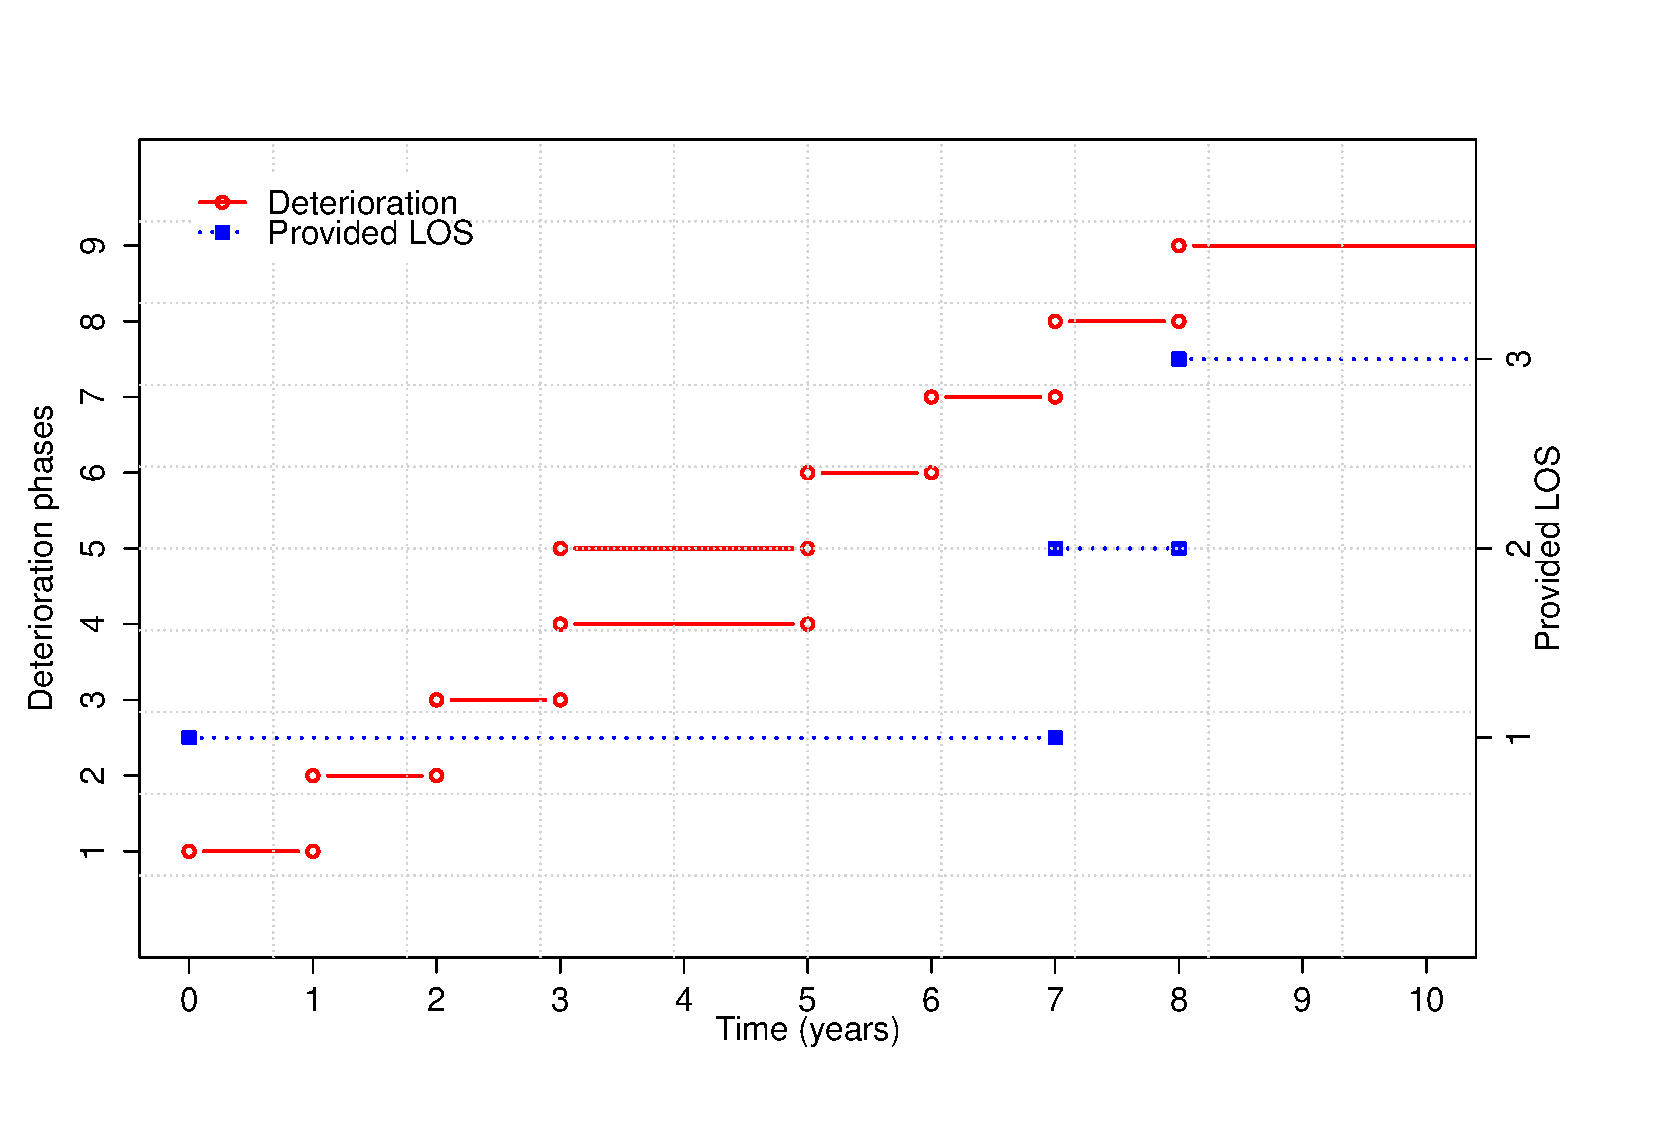
\includegraphics[width=376pt]{fig22.eps}
\caption{Illustration of relationship between deterioration processes and the provided LOS}\label{fig22}
\end{figure}

\subsection{Required LOSs}

Changes in required LOSs are the result of changing human needs. They often result in existing infrastructure providing an inadequate LOS. For example, if a bridge was designed to have two lanes but a decision was made to expand the road to four lanes to accommodate changing human needs, then the bridge would no longer provide an adequate LOS.

From an infrastructure managers perspective, processes that result in changes in required LOSs, as deterioration processes, can be classified as either manifest or latent. 

With respect to changes in required LOSs most processes are considered manifest if development strategies are well developed and triggers for the execution of interventions are determined. For example, the need to expand a road due to it reaching its carrying capacity in terms of number of vehicles in peak periods can be considered as a manifest process if the number of vehicles per hour are recorded every day and a development strategy has been determined that states that once the road is at 80\% its maximum capacity the road will be widened. 

Most processes are considered as latent if development strategies are not well developed and no triggers for the execution of interventions are determined. For example, if the infrastructure manager is focused simply on maintaining the physical condition of the road it may come to him as a surprise when suddenly politicians request that a certain road be widened. 

Some example of processes that can result in changes in the required LOS in buildings can be are shown in Table \ref{tbl:212}.

\begin{table}
\caption{Example changes for buildings and related processes}
\begin{tabular}{|l|l|ll}
\cline{1-2}
Change & Related process &  &  \\ 
\cline{1-2}
Floor space layout & Demand for apartments suitable for growing elderly population &  &  \\ 
\cline{1-2}
New windows & Demand for energy efficient houses and rises.  &  &  \\ 
\cline{1-2}
New heating system & Demand for less maintenance on the heating system &  &  \\ 
\cline{1-2}
New control system & Demand for better control over the quality of the indoor air condition. &  &  \\ 
\cline{1-2}
\end{tabular}
\label{tbl:212}
\end{table}

Changes to the required LOS can happen due the wishes of the owners of infrastructure or be imposed by external persons such as government. The government can also provide incentives for the owner to change the required LOS. Other stakeholders can exert influence on the owner to change the required LOS, e.g. tenants in an apartment building can threaten not to pay the rent unless an air conditioning system is installed. The development of new technologies can also instigate changes in the required LOS as new developments may make things possible that were not before, e.g. new heating systems.

\subsection{Methodology}

The five basic steps to modelling changes in the required LOS are (adapted from \cite{Neufville2011}):

\begin{itemize}
	\item \underline{Step 1}:  Identify key performance drivers, i.e. determine the things that if changed will result in a change in the required LOS, e.g. if the number of vehicles per day pass x, then the road will need to be widen.
	\item \underline{Step 2}: Analyse historical trends, i.e. obtain as much historical data as possible and model how it changed over time with the plan to use this model to predict the future values, e.g. obtain the evolution of vehicles on the road over the last 20 years.
	\item \underline{Step 3}: Identify trend breakers, i.e. dig deeper and try to determine if there is something that can be used to help you predict if this trend will continue or might change suddenly, e.g. a new rail link on which passenger trains will circulate is about to be completed where there was none before.
	\item \underline{Step 4}: Establish forecast accuracy, i.e. if enough data exists put yourself mentally in the past and see how could you have predicted the future for which you have data, e.g. using only traffic data from 1980 to 1999 how could would you be at predicting the traffic between 2000 and 2014. 
	\item \underline{Step 5}: Build a dynamic model, i.e. build a model that allows a range of predictions to be made using a sensible distribution. 
\end{itemize}

An example for a hospital is provided in  the work of \cite{Neufville2011} . 

More detail on model development will be provided later.

\section{Change in LOS-Example}

\subsection{Question C}

Using the owner and user impacts of the impact hierarchy developed in section 3, develop simple models to be used to estimate how the provided LOS of a road will change over 20 years to the relatively slow deterioration of the pavement surface. 

\subsection{Answer C}

\subsubsection{Background}

In order to develop simple models to quantify the values of the various impact types it is useful to think of the object under investigation as being in one of two states, i.e. when no intervention is being executed and when an intervention is being executed. In general, these can be represented by the functions $f_{}^k(t,x)$ and $g_{}^k(d,x)$, respectively (here, \textit{k} represents intervention to be executed, e.g. renewal of the road section; \textit{x} represents the performance indicator, \textit{t} and \textit{d} represent in between interventions and during intervention, respectively). It is assumed that they are expressed in \textit{mus}. Both can be given by functions that vary over time. For example, two following generic exponential functions which can be used are: 

\begin{eqnarray}
      && {f^k}(t,x) = {a^{k,x}} + {b^{k,x}} \cdot \exp ({\beta ^{k,x}} \cdot t) \label{fx}\\
      && {g^k}(d,x) = {\bar a^{k,x}} + {\bar b^{k,x}} \cdot \exp ({\bar \beta ^{k,x}} \cdot {d^k}) \label{gx}
\end{eqnarray}


Where  or ${f^k}(t,x)$ and $g_{}^k(d,x)$ represent the impacts (costs) that are incurred as a function of time (\textit{t} or \textit{d}) and parameters $a$, $b$, and $\beta $.

If it is assumed that the change in condition of the road over time is known, this equation links the changes any impact on any stakeholder to the change in condition of the road over time.  

An example of the evolution of vehicle operation cost (VoC) along with the evolution of roughness for 1 m length of road is shown in Figure \ref{fig23}. In the figure, Eq. (1) has parameter values \textit{a}=500, \textit{b}=800, and $\beta  = 0.095$. These values are often estimated using empirical models. For example, in order to estimate the evolution of the VoC in between two consecutive interventions (from ${t_1}$ to ${t_2}$), \cite{Ouyang2004} used the following function.

\begin{eqnarray}
      && \int\limits_{{t_1}}^{{t_2}} {{f^k}\left[ {s(t)} \right]} {e^{ - rt}}dt = c\int\limits_{{t_1}}^{{t_2}} {s(t){e^{ - rt}}} dt \label{stx}
\end{eqnarray}

In Eq. \eqref{stx}, $s(t)$ represents the roughness indicators; c is constant associated with cost; $r$ is discount factor. The functional form of the roughness can be estimated with a simple exponential function as follows:

\begin{eqnarray}
      && s(t) = s({t_0}) \cdot \exp \left[ {\alpha (t - {t_0})} \right] \hspace{2mm} (for \hspace{2mm} t \ge {t_0}) \label{stx1}
\end{eqnarray}


Where $s({t_0})$ is initial roughness indicator (the initial LOS) and $\alpha $is a deterioration parameter.

When the time \textit{t} is discrete, \cite{Ouyang2004} suggests to use following function

\begin{eqnarray}
      && s(t + 1) = \left[ {s(t) + \upsilon } \right] \cdot \exp (\alpha ) \label{stx2}
\end{eqnarray}

With $\upsilon $ is the pre-defined model's parameter.

The cost curve (green curve in Figure \ref{fig23}) represents the increase of vehicle operation cost over time. The discount rate used is 2\%. Evolution of roughness is estimated from using Eq. \eqref{stx2} with $\upsilon  = 2$ and $\alpha  = 0.0153$. Value of parameter $c$in Eq. \eqref{stx} is 2.1.

\begin{figure}[h]
\begin{center}
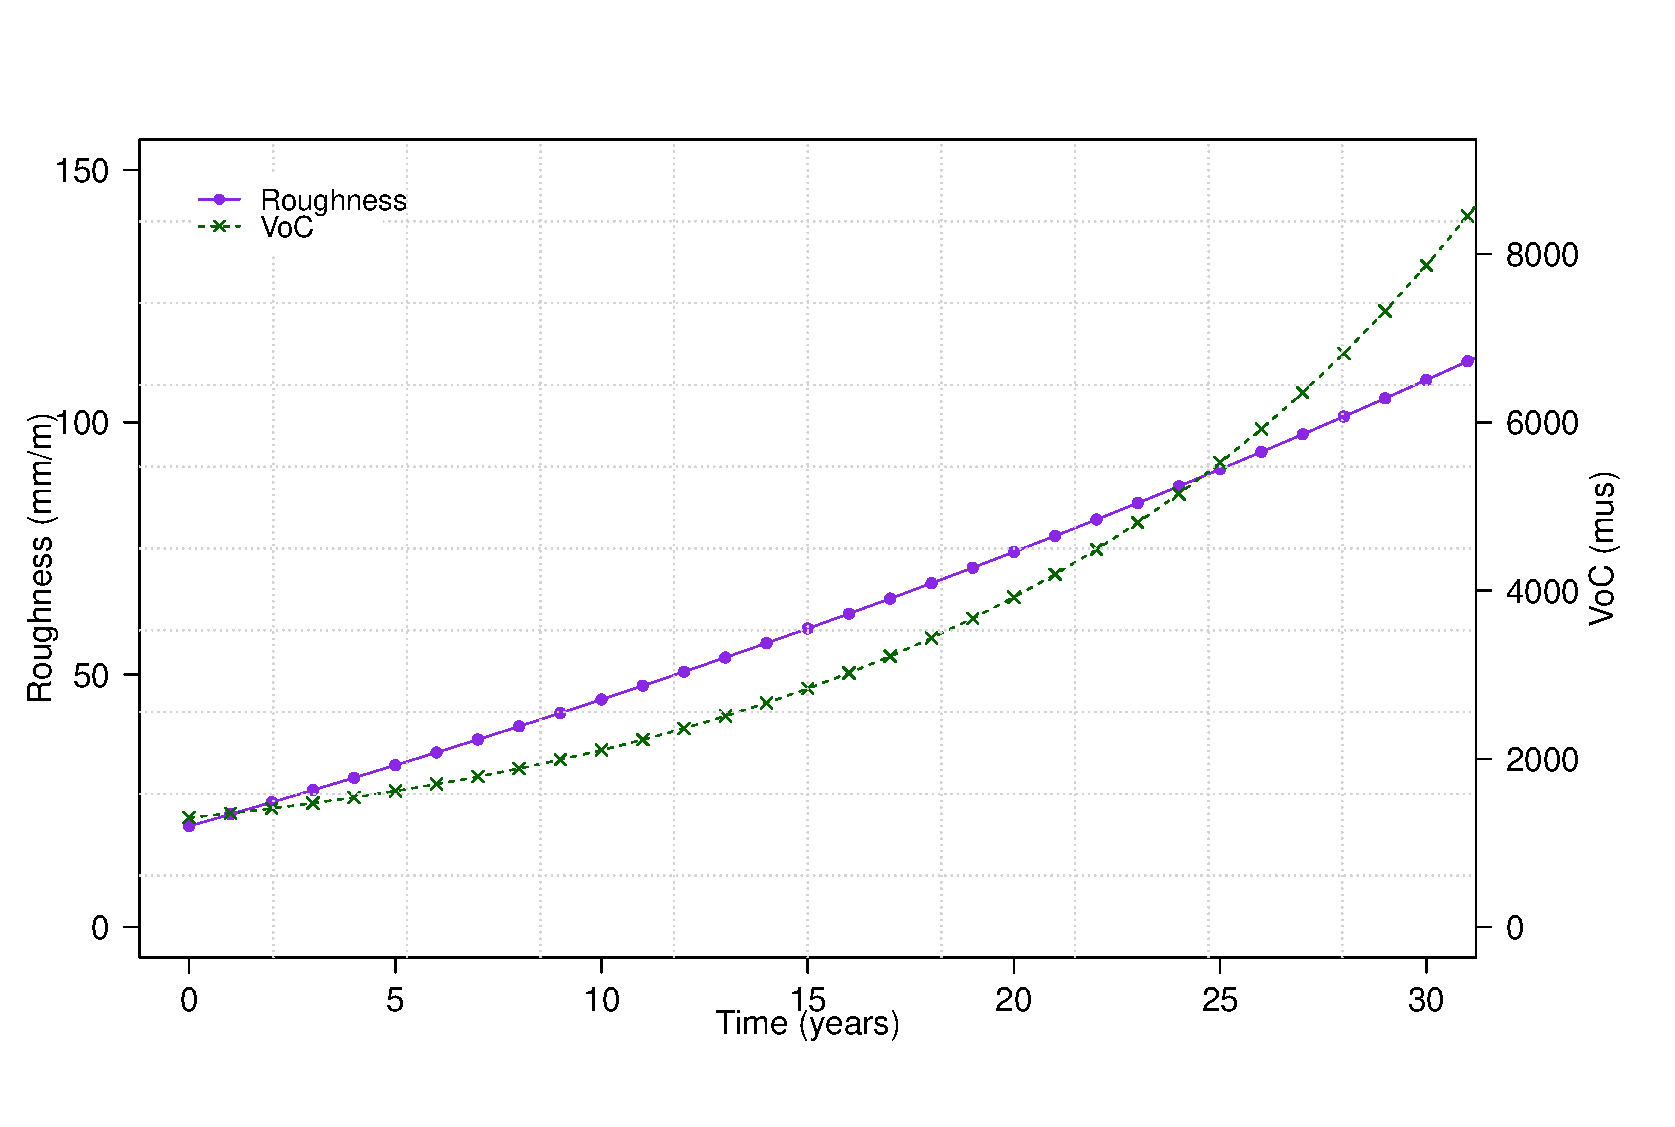
\includegraphics[width=402pt]{fig23.eps}
\caption{Evolution of VoC and roughness indicator}\label{fig23}
\end{center}
\end{figure}
 
Being generic, Eqs. \eqref{fx} and \eqref{gx} can be used to model the evolution of any impact that varies as a function of the condition of a road section, and allows the heterogeneity of each road section, e.g. the different deterioration rates, to be taken into consideration. For example, if it is desired to model the relationship between impacts on the user and the condition of a road section, the values of a, b, and \textit{$\beta{}$} (e.g. for user) could be selected as non-negative values, ensuring that the function \textit{f }will result in the values of the impact on the users that increase exponentially with time. This is similar to that of the user cost estimated using Eq. \eqref{stx}. Although the form of functions \textit{f} and \textit{g} are flexible, here, the exponential form is often used. 
%%%
\subsubsection{Owner}
%%%
\begin{eqnarray}
      && f_{}^k(t,x_i^o) = \sum\limits_{i = 1}^3 {I_i^o(t) \cdot c_i^o(t)} \label{fx1}\\
      && g_{}^k(d,x_i^o) = \sum\limits_{j = 1}^3 {I_i^o(d) \cdot c_i^o(d)} \label{gx1}
\end{eqnarray}
Where:\\
%\begin{flushright}
\begin{adjustwidth}{1cm}{}
\begin{description}
\item[$i$:] is the index of impact types: labor, equipment, and materials
\item[$I_i^o$:] is the owner impact indicator for impact type i. In this case it is the number of person-hours, numbers of equipment use hours, and quantity of materials used for intervention
\item[$c_i^o(t)$ and $c_i^o(d)$:] are owner unit costs, which vary as a function of time $t$ and $d$
\end{description}
%\end{flushright}
\end{adjustwidth}
\subsubsection{Users}
\begin{eqnarray}
      && f_{}^k(t,x_i^u) = \sum\limits_{i = 1}^3 {I_i^u(t) \cdot c_i^u(t)} \label{fx2}\\
      && g_{}^k(d,x_i^u) = \sum\limits_{i = 1}^3 {I_i^u(d) \cdot c_i^u(d)} \label{gx2}
\end{eqnarray}
Where:
%\begin{flushright}
\begin{adjustwidth}{1cm}{}
\begin{description}
\item[$i$:] is the index of impact types
\item[$I_i^u$:] is the user impact indicator for impact type $i$ 
\item[$c_i^u(t)$ and $c_i^u(d)$:] are user unit costs, which vary as a function of time $t$ and $d$.
\end{description}
%\end{flushright}
\end{adjustwidth}
%%%
\paragraph{\underline{Safety}}
The values of impact indicators ($I_i^u(t)$and $I_i^u(d)$) are generally estimated through regression analysis using empirical models. In empirical models, values of impact indicators associated with accidents can be estimated by using the ``accident rate'' multiplied by the cost of the accidents if they occur. Both depend on multiple factors such as the condition of the road, daily traffic volume, the physical condition of the driver of the vehicle and environmental factors such as, the occurrence of poor weather that can effect accident rate. For example, a popular way to estimate the value of impact indicators is by use of following equation \citep{Lindenmann2008}.

\begin{eqnarray}
      && I_{property}^u = t \cdot DTV \cdot s \cdot \theta  \cdot \omega  \cdot \upsilon \label{safety1}
\end{eqnarray}
Where:
%\begin{flushright}
\begin{adjustwidth}{1cm}{}
\begin{description}
\item[$t$:] is the number of days,
\item[$DTV$:] is the daily traffic volume,
\item[$s$:] is the length of the object,
\item[$\theta$:] is the coefficient depending on the deterioration level of the civil infrastructure,
\item[$\omega$:] is the correction factor for accident rate, and
\item[$\upsilon$:] is the approximate numbers of vehicles involved in an accident.
\end{description}
%\end{flushright}
\end{adjustwidth}
According to \cite{tarko2000}, three ways commonly used to estimate the accident rate are 
\begin{enumerate}
	\item crash rate method, which recommends a rate of crash for a specific type of road, in specific location, and with specified level of traffic volume; 
	\item crash equation method, which relies on a functional form of traffic volume and engineering factors; 
	\item crash reduction factor method, which is an extension method of crash equation method, where the crash reduction factor is given by: 
\end{enumerate}

\begin{eqnarray}
      && f(X) = k \cdot Y \cdot {Q^\gamma } \cdot {e^{\beta x}} \label{safety2}
\end{eqnarray}
Where:
\begin{adjustwidth}{1cm}{}
\begin{description}
\item[$f(X)$:] is the crash reduction function,
\item[$k$:] is a constant,
\item[$Y, Q$:] are the exposure variables representing the temporal span of data and indicate the section length and traffic volume, respectively, 
\item[$\beta$:] is the an unknown parameter associated with the variable X.
\item[$X$:] is the variable vector of engineering factors, including the performance condition of the road.
\end{description}
%\end{flushright}
\end{adjustwidth}
After obtaining the accident rate related to the execution of an intervention for each intervention type on an each object (i.e. between and during interventions), the value of impact indicators $I_i^u(t)$ and can be calculated. 

For example, after the execution of an intervention, an asphalt road section of 20 km is renewed to be in condition state 1. The daily traffic volume is 600 vehicles/day. The accident rates during and after intervention are estimated to be 0.03\% and 0.005\% out of the total traffic volume in a day. The duration of the intervention is 30 days. It is assumed that the average number of vehicles involved in an accident are two. 
%
The expected total numbers of vehicles involved in accidents in a year after intervention will be:

$I^u_{property}(t=365) \hspace{1mm}days \hspace{1mm} =365\times600\times0.005\%\times2 \approx 22 \hspace{1mm}$ vehicles 
%

The expected total numbers of vehicles involved in accidents during intervention will be:

$I^u_{property}(d=30) \hspace{1mm}days \hspace{1mm} =30\times600\times0.03\%\times2 \approx 11 \hspace{1mm}$ vehicles

The average unit cost $c_{{\rm{property}}}^u(t)$per vehicle can be approximated from historical data \cite{Lindberg1999}. 

\paragraph{\underline{Operation efficiency}}

The values of the travel time impact indicator can be approximated as a function of multiple factors including vehicle speed, amount of congestion, and curviness of the road. 

The values of the vehicle operation and maintenance impact indicators can be approximated as a function of multiple factors including the total number of vehicle type \textit{j}. (type $j$ means type of vehicles such as car, truck, bus, etc), 
\begin{eqnarray}
      && f^{k_{n_l}}_{n_l}(t,x^u_i)=I^u_{i,k_{n_l}} = \sum_{i=1}^2\sum_{j=1}^J C^u_{ij}(t) \cdot VH_j (t) \label{operation1}\\
      && g^{k_{n_l}}_{n_l}(d,x^u_i)=I^u_{i,k_{n_l}} = \sum_{i=1}^2\sum_{j=1}^J C^u_{ij}(d) \cdot VH_j (d) \label{operation2}
\end{eqnarray}
Where:
\begin{adjustwidth}{1cm}{}
\begin{description}
\item[$I_i^u$:] is the impact indicator for the index \textit{i}
\item[$i$:] is the index for vehicle maintenance cost and vehicle operation cost.
\item[$VH$:] is total number of vehicle type \textit{j}. (type \textit{\underline{j}} means type of vehicles such as car, truck, bus, etc). The value of \textit{VH} can be obtained from examining historical record on traffic volume and annual growth of traffic volume.
\end{description}
%\end{flushright}
\end{adjustwidth}
%
The value of $C_{ij}^u(t)$can be estimated by empirical study or regression analysis based on recorded numbers of bill paid for operation and maintenance respectively. To date, several models have been developed to relate such cost to deterioration or performance of the road. For example,\cite{OpusCL1999} studied the relationship between vehicle operation cost and international roughness index. The value of \textit{VH} can be obtained from examining historical record on traffic volume and annual growth of traffic volume.
%
\paragraph{\underline{Operational Quality}}
Impact indicators associated with and  can be measured by using qualitative scale (e.g, scale from 1 to 5, with 1 is the best and 5 is the worst) or by carrying out an empirical study on the loss in effective working time if users travel on a target road link. The values of the differences between these states in these scales can be determined through willing to pay investigations. 

Following proposed function can be used for estimating the values of impact indicators $BI^u_{physical, k_{n_l}}$ and $BI^u_{psychological, k_{n_l}}$.
\begin{eqnarray}
      && BI^u_{i,k_{n_l}} = t\cdot U\cdot \mu_i \label{operation3}
\end{eqnarray}
Where:
\begin{adjustwidth}{1cm}{}
\begin{description}
\item[$t$:] is the number of days,
\item[$U$:] is expected number of users per day, which can be approximated by means of daily traffic volume,
\item[$\mu$:] is the mean value of amount of physical and psychological impacts. It can be obtained by carrying out surveys on a population sample of the users.
\end{description}
%\end{flushright}
\end{adjustwidth}

For example, a survey using qualitative method on 300 users, who travel on a certain road link of 20 km, reveals a mean value $\mu_{physical}=3.4$ (from a scale of 5) per 1 km. The daily users have a factor of 2.5 times the daily traffic volume, which is 600 vehicles/day. Thus, in 30 days, the values of $I^u_{physical}=3.4$ will be determined as:

$I^u_{physical} = 30 \times (600 \times 2.5) \times 3.4 = 153'000 $ units

If each unit of physical impact is relatively cost 0.05 $mus$, then in total 30 days, the cost incurred to users due to physical impact will be $0.05(mus/unit)\times 153'000 (units)=7'650$  (mus).

\paragraph{Environment preservation (reduction of noise)}

Impact indicators associated with $I_{noise}^u$ can be approximated by use of following equation.

\begin{eqnarray}
      && I^u_{noise} = t\cdot \overline{dBA} \cdot U \label{operation4}
\end{eqnarray}
Where:
\begin{adjustwidth}{1cm}{}
\begin{description}
\item[$t$:] are the number of days in between interventions and during intervention,
\item[$\overline{dBA}$:] is the expected increase unit of noise (in $dBA$).
\item[$U$:] is the expected number of users within a specific period.
\end{description}
%\end{flushright}
\end{adjustwidth}

For example, an intervention is scheduled to last 30 days. The expected numbers of users could be estimated as 300 persons. If during intervention, the noise due to construction activities increases by 2 $dBA$ compared to the normal day without intervention, and one additional dBA has a value of 100 mus. Using Eq. \eqref{operation4}, the values of impact indicator will be

$I^u_{noise}=30 \times 2 \time 300 = 18'000 dBA-person-days$

and thus, the values of function $g^d(d,x^u_{noise})$ will be 

$g^d(d,x^u_{noise}) = 18'000 \times 100 = 1'800'000 \hspace {1mm} mus$
%
\section{Assignments}
\subsection{Problem A}
In class an impact hierarchy was given to be used to determine optimal intervention strategies and work programs for a road network. Discuss the suitability of this impacts hierarchy if it was to be used to determine optimal intervention strategies and work programs for 
\begin{adjustwidth}{1cm}{}
\begin{itemize}
\item[a)] a private road network, and 
\item[b)] a public rail network.                         
\end{itemize}
\end{adjustwidth}
%
\subsection{Answer A-a}
No specific answer is provided. Please submit your answer to obtain feedback. 
\subsection{Answer A-b}
No specific answer is provided. Please submit your answer to obtain feedback. 
%
\subsection{Problem B}
Water is one of the fundamental needs of millions of people living in a megacity. Water of sufficient quality and quantity must be provided around the clock. In order to fulfill this need, a city depends on its water distribution infrastructure, which includes pipes made of different materials and laid at different times. These pipes are affected by processes of different types and deteriorate at different rates. The consequences related to pipe failure vary significantly depending on the type of failure, e.g. a pipe break, or a leaking pipe, as does the reaction time required to fix the pipe. For example, if a pipe breaks, a corrective intervention must be executed immediately, and if it is noticed that there is progressive water loss over time then a preventive intervention can be planned before there is an inadequate level of service.  Part of the water distribution network in mega-city Q is shown in Figure \ref{fig24}. The pipe characteristics are given in Table \ref{tbl:213}. 

\begin{figure}[h]
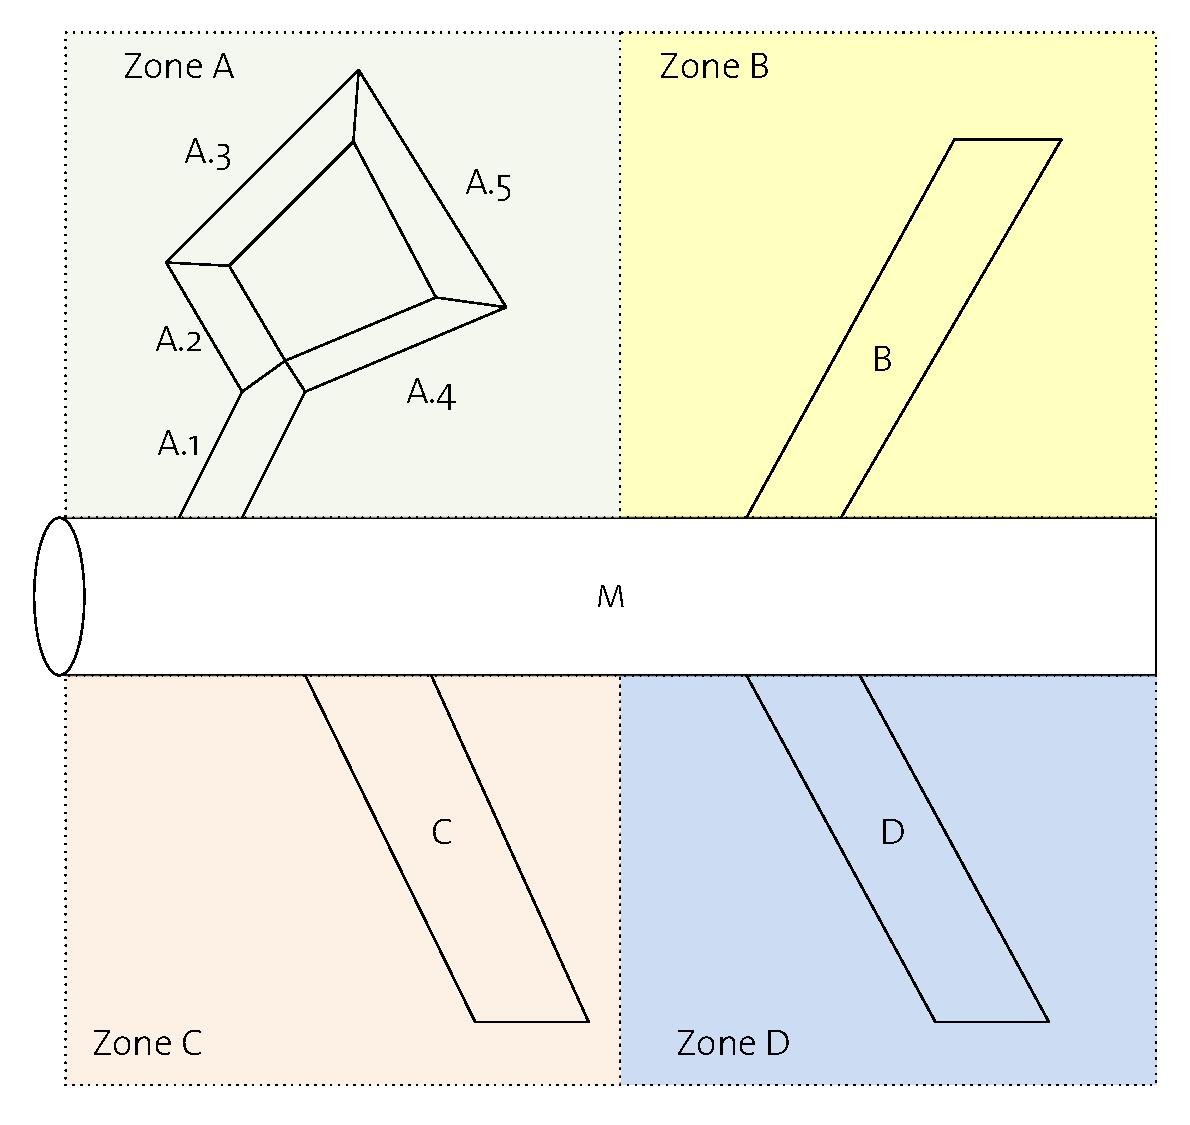
\includegraphics[width=200pt]{fig24.eps}
\caption{Simplified network of water supply pipes}\label{fig24}
\end{figure}


\begin{table}
\caption{Pipe and their attributes}
\begin{tabular}{|l|l|l|l|l|p{80pt}|}
\hline
\multicolumn{1}{|c|}{Pipe} & Material & \multicolumn{1}{c|}{Demand (m3/day)} & \multicolumn{1}{c|}{Length (m)} & \multicolumn{1}{c|}{Year of construction} & Usage \\ 
\hline
\multicolumn{1}{|c|}{M} & Concrete & \multicolumn{1}{c|}{} & \multicolumn{1}{c|}{5'000} & \multicolumn{1}{c|}{1998} & Distribution only \\ 
\hline
\multicolumn{1}{|c|}{A.1} & PVC & \multicolumn{1}{c|}{250'000} & \multicolumn{1}{c|}{600} & \multicolumn{1}{c|}{2003} & Distribution only \\ 
\cline{1-2}\cline{4-6}
\multicolumn{1}{|c|}{A.2} & PVC & \multicolumn{1}{c|}{} & \multicolumn{1}{c|}{600} & \multicolumn{1}{c|}{2003} & Distribution only \\ 
\cline{1-2}\cline{4-6}
\multicolumn{1}{|c|}{A.3} & PVC & \multicolumn{1}{c|}{} & \multicolumn{1}{c|}{600} & \multicolumn{1}{c|}{2003} & Distribution and connection to buildings \\ 
\cline{1-2}\cline{4-6}
\multicolumn{1}{|c|}{A.4} & PVC & \multicolumn{1}{c|}{} & \multicolumn{1}{c|}{600} & \multicolumn{1}{c|}{2003} & Distribution only \\ 
\cline{1-2}\cline{4-6}
\multicolumn{1}{|c|}{A.5} & PVC & \multicolumn{1}{c|}{} & \multicolumn{1}{c|}{600} & \multicolumn{1}{c|}{1998} & Distribution and connection to buildings \\ 
\hline
\multicolumn{1}{|c|}{B} & Cast iron type 1 & \multicolumn{1}{c|}{200'000} & \multicolumn{1}{c|}{2'500} & \multicolumn{1}{c|}{1993} & Distribution and connection to buildings \\ 
\hline
\multicolumn{1}{|c|}{C} & Cast iron type 2 & \multicolumn{1}{c|}{100'000} & \multicolumn{1}{c|}{1'600} & \multicolumn{1}{c|}{1993} & Distribution and connection to buildings \\ 
\hline
\multicolumn{1}{|c|}{D} & Cast iron type 3 & \multicolumn{1}{c|}{350'000} & \multicolumn{1}{c|}{4'000} & \multicolumn{1}{c|}{1983} & Distribution and connection to buildings \\ 
\hline
\end{tabular}
\label{tbl:213}
\end{table}
%
\subsection{Question B}
Make an impact hierarchy that you would use to measure the performance of the network. Be complete at the highest level, i.e. the stakeholders, and be detailed for one of the stakeholders besides the owner.
\subsection{Answer B}
No specific answer is provided. Please submit your answer to obtain feedback. 
\subsection{Problem C}
\subsection{Question C}
Using the impact hierarchy for public roads in the script explain three processes that would result in a change in a required level of service defined using accident costs, travel time costs and maintenance costs. 
\subsection{Answer C}
No specific answer is provided. Please submit your answer to obtain feedback. 
%
\bibliographystyle{plainnat}
\bibliography{reference}

